\documentclass[border=10pt]{standalone}
\usepackage{tikz}
\usetikzlibrary{shapes.geometric, arrows.meta, positioning, fit, backgrounds, shadows}

\begin{document}

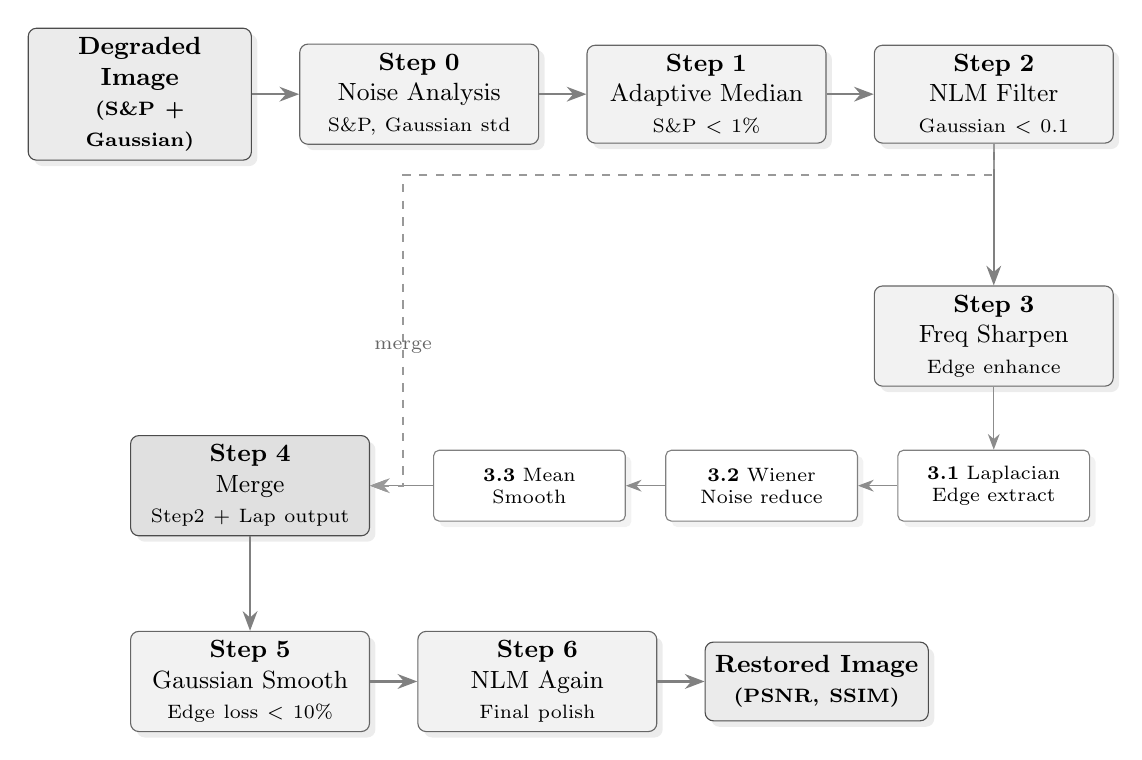
\begin{tikzpicture}[
    node distance=1.0cm and 0.6cm,
    % Professional Gray Styles
    inputbox/.style={rectangle, rounded corners=3pt, draw=black!70, fill=black!8, 
        text width=2.6cm, minimum height=1cm, align=center, font=\small\bfseries,
        drop shadow={opacity=0.15}},
    stepbox/.style={rectangle, rounded corners=3pt, draw=black!60, fill=black!5, 
        text width=2.8cm, minimum height=1.2cm, align=center, font=\small,
        drop shadow={opacity=0.15}},
    substep/.style={rectangle, rounded corners=2pt, draw=black!50, fill=white, 
        text width=2.2cm, minimum height=0.9cm, align=center, font=\scriptsize,
        drop shadow={opacity=0.1}},
    mergestep/.style={rectangle, rounded corners=3pt, draw=black!70, fill=black!12, 
        text width=2.8cm, minimum height=1.2cm, align=center, font=\small,
        drop shadow={opacity=0.15}},
    outputbox/.style={rectangle, rounded corners=3pt, draw=black!70, fill=black!8, 
        text width=2.6cm, minimum height=1cm, align=center, font=\small\bfseries,
        drop shadow={opacity=0.15}},
    arrow/.style={-{Stealth[length=2.5mm]}, thick, draw=black!50},
    dasharrow/.style={-{Stealth[length=2.5mm]}, thick, draw=black!40, dashed},
    subarrow/.style={-{Stealth[length=2mm]}, draw=black!45},
]

% ============ ROW 1: Input and Steps 0-2 ============
\node[inputbox] (input) {Degraded Image\\{\scriptsize(S\&P + Gaussian)}};

\node[stepbox, right=of input] (step0) {\textbf{Step 0}\\Noise Analysis\\{\scriptsize S\&P, Gaussian std}};

\node[stepbox, right=of step0] (step1) {\textbf{Step 1}\\Adaptive Median\\{\scriptsize S\&P $<$ 1\%}};

\node[stepbox, right=of step1] (step2) {\textbf{Step 2}\\NLM Filter\\{\scriptsize Gaussian $<$ 0.1}};

% ============ ROW 2: Step 3 with sub-steps ============
\node[stepbox, below=1.8cm of step2] (step3) {\textbf{Step 3}\\Freq Sharpen\\{\scriptsize Edge enhance}};

% Sub-steps (3.1, 3.2, 3.3) below Step 3
\node[substep, below=0.8cm of step3] (step31) {\textbf{3.1} Laplacian\\{\scriptsize Edge extract}};
\node[substep, left=0.5cm of step31] (step32) {\textbf{3.2} Wiener\\{\scriptsize Noise reduce}};
\node[substep, left=0.5cm of step32] (step33) {\textbf{3.3} Mean\\{\scriptsize Smooth}};

% ============ ROW 3: Steps 4-6 and Output ============
\node[mergestep, left=0.8cm of step33] (step4) {\textbf{Step 4}\\Merge\\{\scriptsize Step2 + Lap output}};

\node[stepbox, below=1.2cm of step4] (step5) {\textbf{Step 5}\\Gaussian Smooth\\{\scriptsize Edge loss $<$ 10\%}};

\node[stepbox, right=of step5] (step6) {\textbf{Step 6}\\NLM Again\\{\scriptsize Final polish}};

\node[outputbox, right=of step6] (output) {Restored Image\\{\scriptsize(PSNR, SSIM)}};

% ============ Main Flow Arrows ============
\draw[arrow] (input) -- (step0);
\draw[arrow] (step0) -- (step1);
\draw[arrow] (step1) -- (step2);
\draw[arrow] (step2) -- (step3);

% Step 3 to sub-steps
\draw[subarrow] (step3) -- (step31);
\draw[subarrow] (step31) -- (step32);
\draw[subarrow] (step32) -- (step33);
\draw[subarrow] (step33) -- (step4);

% Continue main flow
\draw[arrow] (step4) -- (step5);
\draw[arrow] (step5) -- (step6);
\draw[arrow] (step6) -- (output);

% ============ Special Connection: Step 2 to Step 4 (Merge) ============
\draw[dasharrow] (step2.south) -- ++(0,-0.4) -- ++(-7.5,0) |- (step4.east) 
    node[pos=0.25, below, font=\scriptsize, text=black!60] {merge};

\end{tikzpicture}

\end{document}
